% VUT FIT MITAI
% MSZ 2021/2022
% Author: Vladimir Dusek
% Login: xdusek27

%%%%%%%%%%%%%%%%%%%%%%%%%%%%%%%%%%%%%%%%%%%%%%%%%%%%%%%%%%%%%%%%%%%%%%%%%%%%%%%%

% Path to figures
\graphicspath{{pds/architektura_prepinacu}}

%%%%%%%%%%%%%%%%%%%%%%%%%%%%%%%%%%%%%%%%%%%%%%%%%%%%%%%%%%%%%%%%%%%%%%%%%%%%%%%%

\chapter{PDS -- Základní architektury přepínačů, algoritmy pro plánování, řešení blokování, vícestupňové
přepínací sítě.}

%%%%%%%%%%%%%%%%%%%%%%%%%%%%%%%%%%%%%%%%%%%%%%%%%%%%%%%%%%%%%%%%%%%%%%%%%%%%%%%%

\section{Metadata}

\begin{compactitem}
    \item Předmět: Přenos dat, počítačové sítě a protokoly (PDS)
    \item Přednáška:
    \begin{compactitem}
        \item \path{04-switching.pdf}
    \end{compactitem}
    \item Záznam:
    \begin{compactitem}
        \item 2021-03-05
    \end{compactitem}
\end{compactitem}

%%%%%%%%%%%%%%%%%%%%%%%%%%%%%%%%%%%%%%%%%%%%%%%%%%%%%%%%%%%%%%%%%%%%%%%%%%%%%%%%

\section{Úvod a kontext}

\paragraph*{ISO/OSI model} Referenční model ISO/OSI se používá jako názorný příklad řešení komunikace v počítačových a telekomunikačních sítích pomocí vrstevnatého modelu, kde jsou jednotlivé vrstvy nezávislé a snadno nahraditelné. \begin{compactitem}

    \item \textbf{Aplikační vrstva} (L7, \textit{application layer}) \begin{compactitem}
        \item Zajišťuje zpracování dat na nejvyšší úrovni (reprezentace dat, kódování, řízení dialogu, \dots).
        \item Tvořena procesy a aplikacemi, které komunikují po síti.
        \item Bývá slučována s prezentační vrstvou (L6, prezentace dat a šifrování) a relační vrstvou (L5, koordinace a komunikace).
        \item Příklad protokolů: \begin{compactitem}
            \item Uživatelské -- vykonávají služby přímo uživateli (Telnet, SSH, FTP, SMTP, HTTP, \dots)
            \item Systémové -- zajišťují síťové funkce (DNS, DHCP, SNMP, BOOTP, \dots)
        \end{compactitem}
    \end{compactitem}

    \item \textbf{Transportní vrstva} (L4, \textit{transport layer}) \begin{compactitem}
        \item Rozděluje aplikační data (segmentace) na menší jednotky a zapouzdřuje je do segmentů (TCP) / datagramů (UDP).
        \item Vytváří logické spojení mezi procesy (přenáší data konkrétní aplikace ze zdrojového zařízení do aplikace na cílovém zařízení).
        \item Adresace: porty.
        \item Příklad protokolů: TCP, UDP, DCCP, SCTP, MP-TCP, QUIC
    \end{compactitem}

    \item \textbf{Síťová vrstva} (L3, \textit{network layer}) \begin{compactitem}
        \item Zapouzdřuje segmenty/datagramy do paketů.
        \item Řeší směrování.
        \item Adresace: IP adresa (logická adresa).
        \item Příklad protokolů: \begin{compactitem}
            \item IPv4, IPv6
            \item ARP (Address Resolution Protocol), RARP (Reverse ARP) -- Slouží k překladu fyzických adres na IP adresy a obráceně.
            \item ICMP (Internet Control Message Protocol) -- Slouží pro řízení toku a detekce nedosažitelných uzlů.
            \item IGMP (Internet Group Management Protocol)
        \end{compactitem}
    \end{compactitem}

    \item \textbf{Linková vrstva} (L2, \textit{data link layer}, vrstva síťového rozhraní, \textit{network interface layer}) \begin{compactitem}
        \item Zapouzdřuje pakety do rámců.
        \item Zajišťuje \textit{hop-by-hop} doručení.
        \item Adresace: MAC adresa (fyzická adresace).
        \item Příklad protokolů: Ethernet, Token Ring, FDDI, X.25, Frame Relay
    \end{compactitem}

    \item \textbf{Fyzická vrstva} (L1, \textit{physical layer}) \begin{compactitem}
        \item Zajišťuje přenos bitů přes fyzické médium.
    \end{compactitem}
\end{compactitem}

% src: https://linuxhint.com/network-osi-layers-explained
\begin{figure}[H]
    \centering
    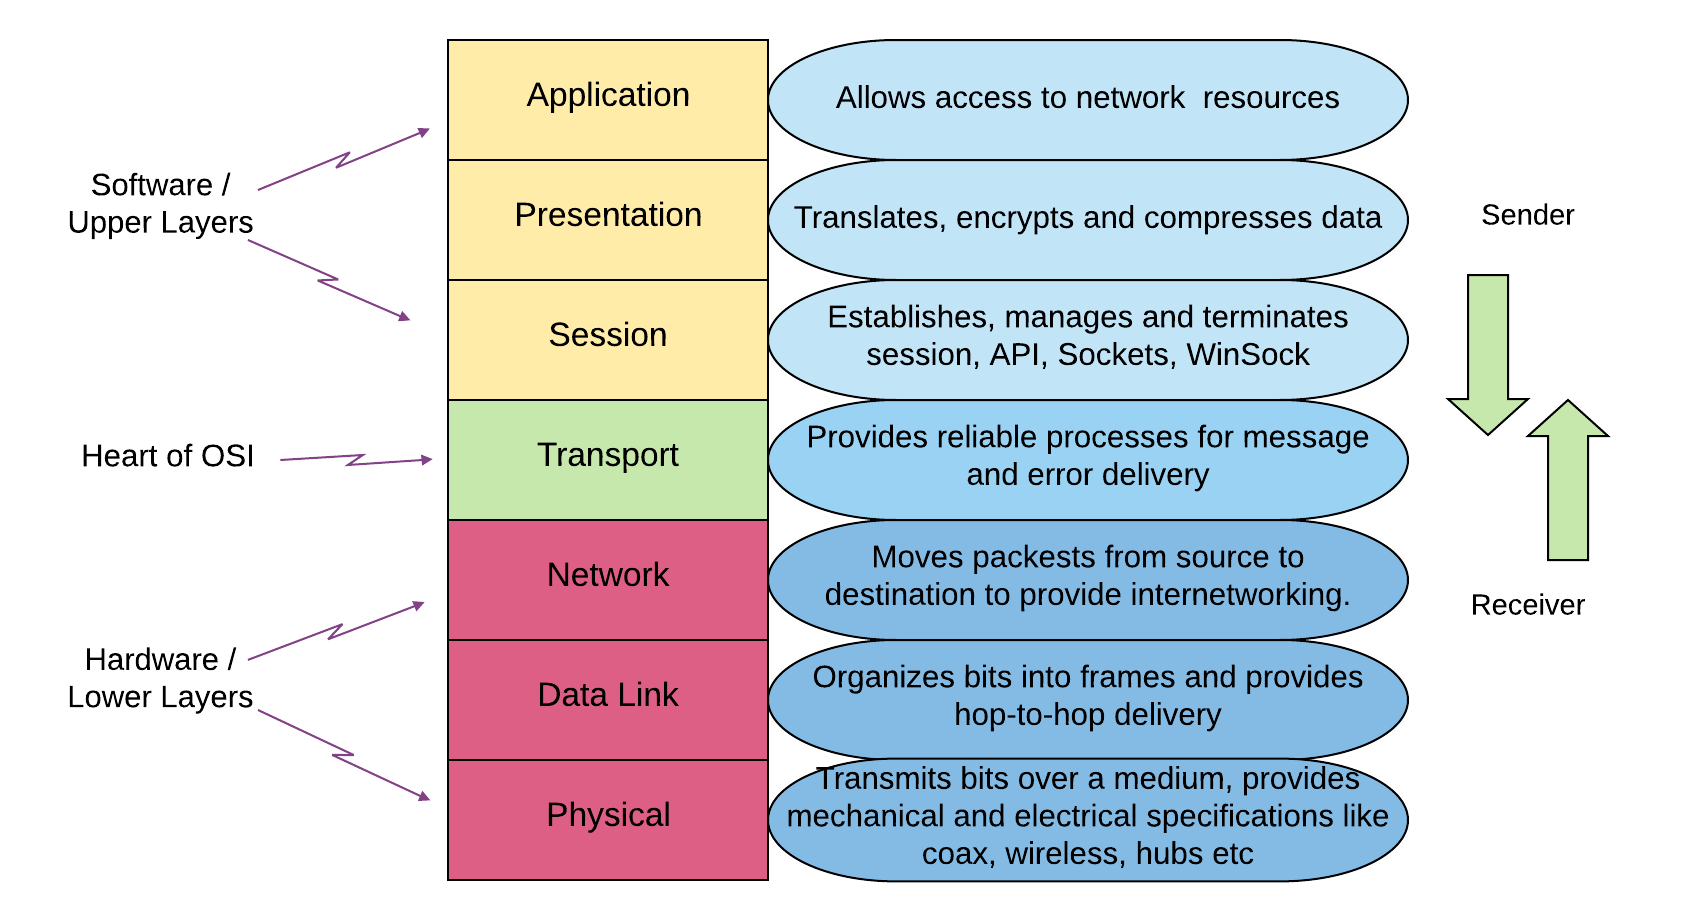
\includegraphics[width=1\linewidth]{osi_model_linuxhint.png}
    \caption{Příklad OSI modelu z Linuxhint.}
\end{figure}

% src: https://cs.wikipedia.org/wiki/Soubor:OSI_Model_v1.svg
\begin{figure}[H]
    \centering
    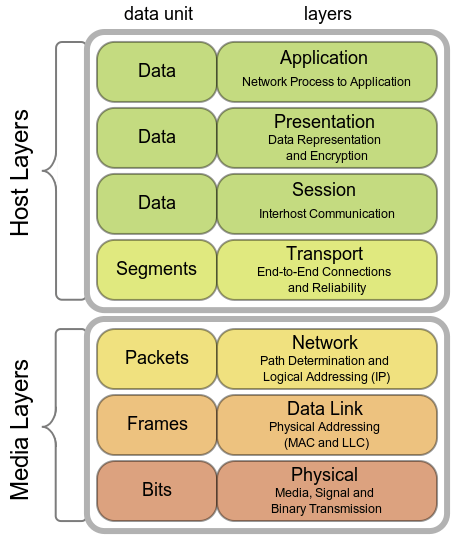
\includegraphics[width=0.65\linewidth]{osi_model_wiki.png}
    \caption{Příklad OSI modelu z Wiki.}
\end{figure}

\paragraph*{Přepínač} Síťový přepínač (\textit{switch}) je aktivní prvek v počítačové síti, který propojuje jednotlivé prvky do hvězdicové topologie. Přepínač obsahuje síťové porty (až stovky), na něž se připojují síťová zařízení. \begin{compactitem}
    \item Na jaké vrstvě OSI modelu pracuje? Pracuje s rámci (linková vrstva, L2).
    \item Na základě čeho provádí přepínání? Na základě cílové MAC adresy.
    \item Jaké typy přenosů přepíná? Na základě cílové MAC adresy rozslišuje typ přenosu: \begin{compactitem}
        \item broadcast (samé 1),
        \item multicast (speciální prefix pro IPv4 a IPv6),
        \item unicast (cokoliv jiného).
    \end{compactitem}
    \item Co ovlivňuje rychlost přepínání? \begin{compactitem}
        \item Hardware (typ paměti, rychlost procesoru)
        \item Logika přepínání
        \item Šířka pásma cílového rozhraní
    \end{compactitem}
\end{compactitem}

\paragraph*{CAM tabulka} Datová struktura v přepínači, ve které se mapují MAC adresy na výstupní porty.

\paragraph*{Problém párování} \todo{todo}

%%%%%%%%%%%%%%%%%%%%%%%%%%%%%%%%%%%%%%%%%%%%%%%%%%%%%%%%%%%%%%%%%%%%%%%%%%%%%%%%

\section{Obecná architektura přepínače}

\begin{figure}[H]
    \centering
    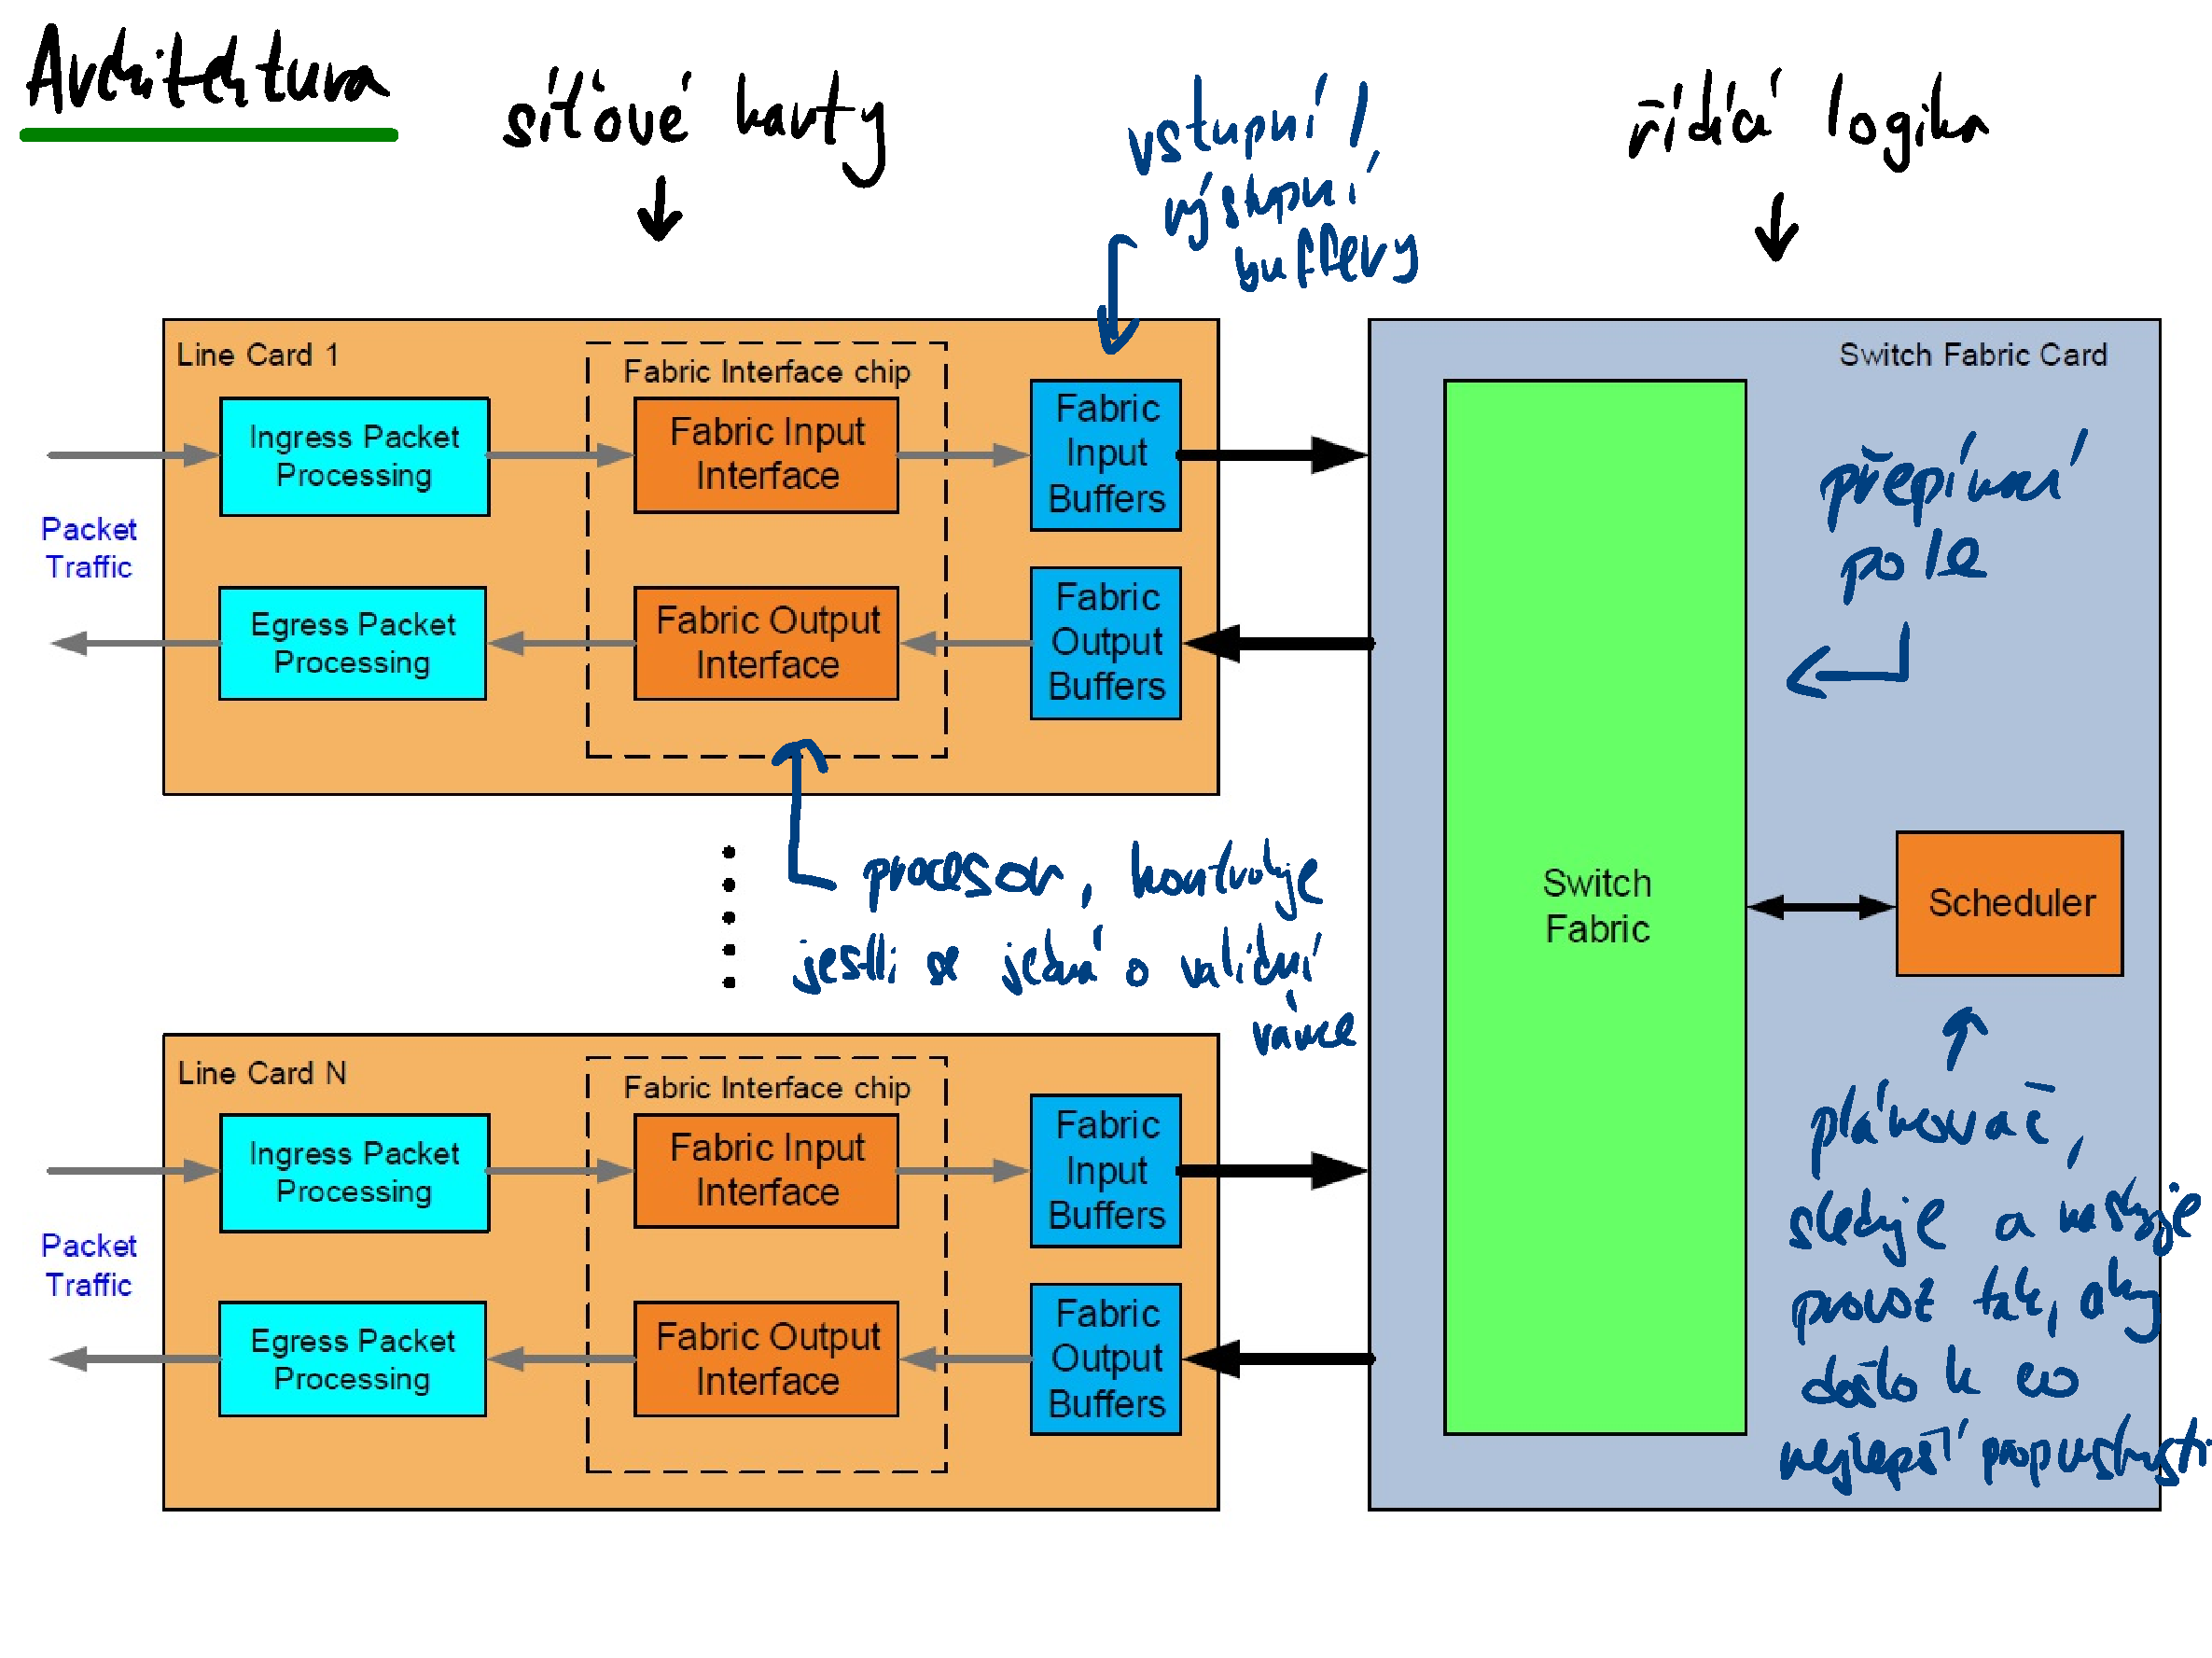
\includegraphics[width=1\linewidth]{obecna_architektura.pdf}
    \caption{Příklad OSI modelu z PDS s příkladem protokolů.}
\end{figure}

\paragraph*{Požadavky na přenos} \begin{compactitem}
    \item Maximální využití sběrnice (požadavek na plánovač). \begin{compactitem}
        \item Aby došlo k maximálnímu přenosu dat přepínací logikou (co nejvíce přenosů v rámci taktu -- \uv{paralelizace}).
    \end{compactitem}
    \item Spravedlivé přidělování přenosového pásma (aby byly obsluhovány všechny porty).
    \item Zachování pořadí rámců (ne vždy vyjde).
\end{compactitem}

\begin{figure}[H]
    \centering
    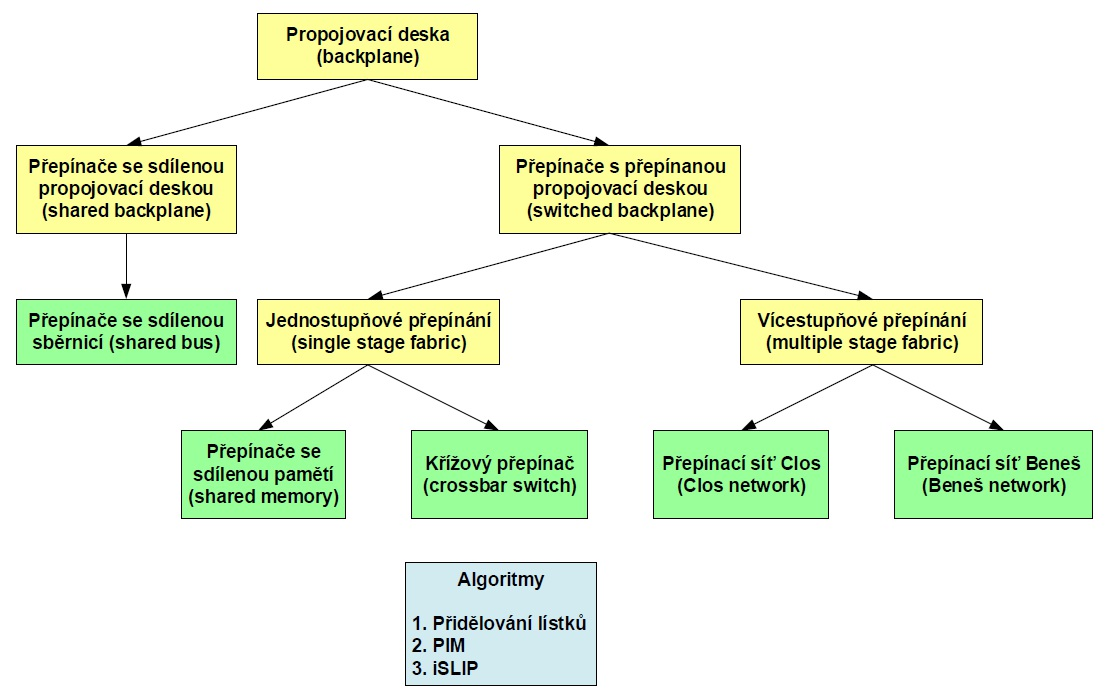
\includegraphics[width=1\linewidth]{deleni_prepinacu.png}
    \caption{Dělení přepínačů.}
\end{figure}

% \paragraph*{Dělení přepínačů} \begin{compactitem}
%     \item Přepínače se sdílenou propojovací deskou (\textit{shared backplane}) \begin{compactitem}
%         \item Přepínače se sdílenou sběrnicí (\textit{shared bus})
%     \end{compactitem}
%     \item Přepínače s přepínanou propojovací deskou (\textit{switched backplane}) \begin{compactitem}
%         \item Jednostupňové přepínání (\textit{single stage fabric}) \begin{compactitem}
%             \item Přepínače se sdílenou pamětí (\textit{shared memory})
%             \item Křížový přepínač (\textit{crossbar switch}) \begin{compactitem}
%                 \item Algoritmus přidělování lístků
%                 \item Algoritmus PIM
%                 \item Algoritmus iSLIP
%             \end{compactitem}
%         \end{compactitem}
%         \item Vícestupňové přepínání \begin{compactitem}
%             \item Přepínací síť Clos
%             \item Přepínací síť Beneš
%         \end{compactitem}
%     \end{compactitem}
% \end{compactitem}

%%%%%%%%%%%%%%%%%%%%%%%%%%%%%%%%%%%%%%%%%%%%%%%%%%%%%%%%%%%%%%%%%%%%%%%%%%%%%%%%

\section{Přepínače se sdílenou propojovací deskou}

\subsection{Přepínače se sdílenou sběrnicí}

\begin{compactitem}
    \item Může komunikovat pouze jeden port v daný čas, ostatní čekají (řízeno protokolem).
    \item Lze jednoduše realizovat broadcast a multicast.
    \item Mějme $N$ portů (karet), rychlost každé karty $R$ bps, taktovací frekvenci $r$. Pak rychlost sběrnice musí být $N \times R$ a šířka sběrnice $$W = \frac{R \times N}{r}$$
\end{compactitem}

\begin{figure}[H]
    \centering
    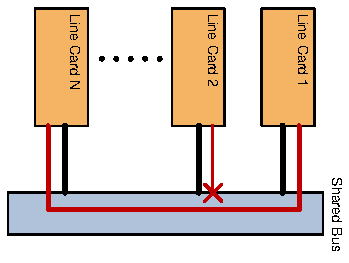
\includegraphics[width=0.5\linewidth]{sdilena_sbernice.pdf}
    \caption{Přepínač se sdílenou sběrnicí.}
\end{figure}

\begin{figure}[H]
    \centering
    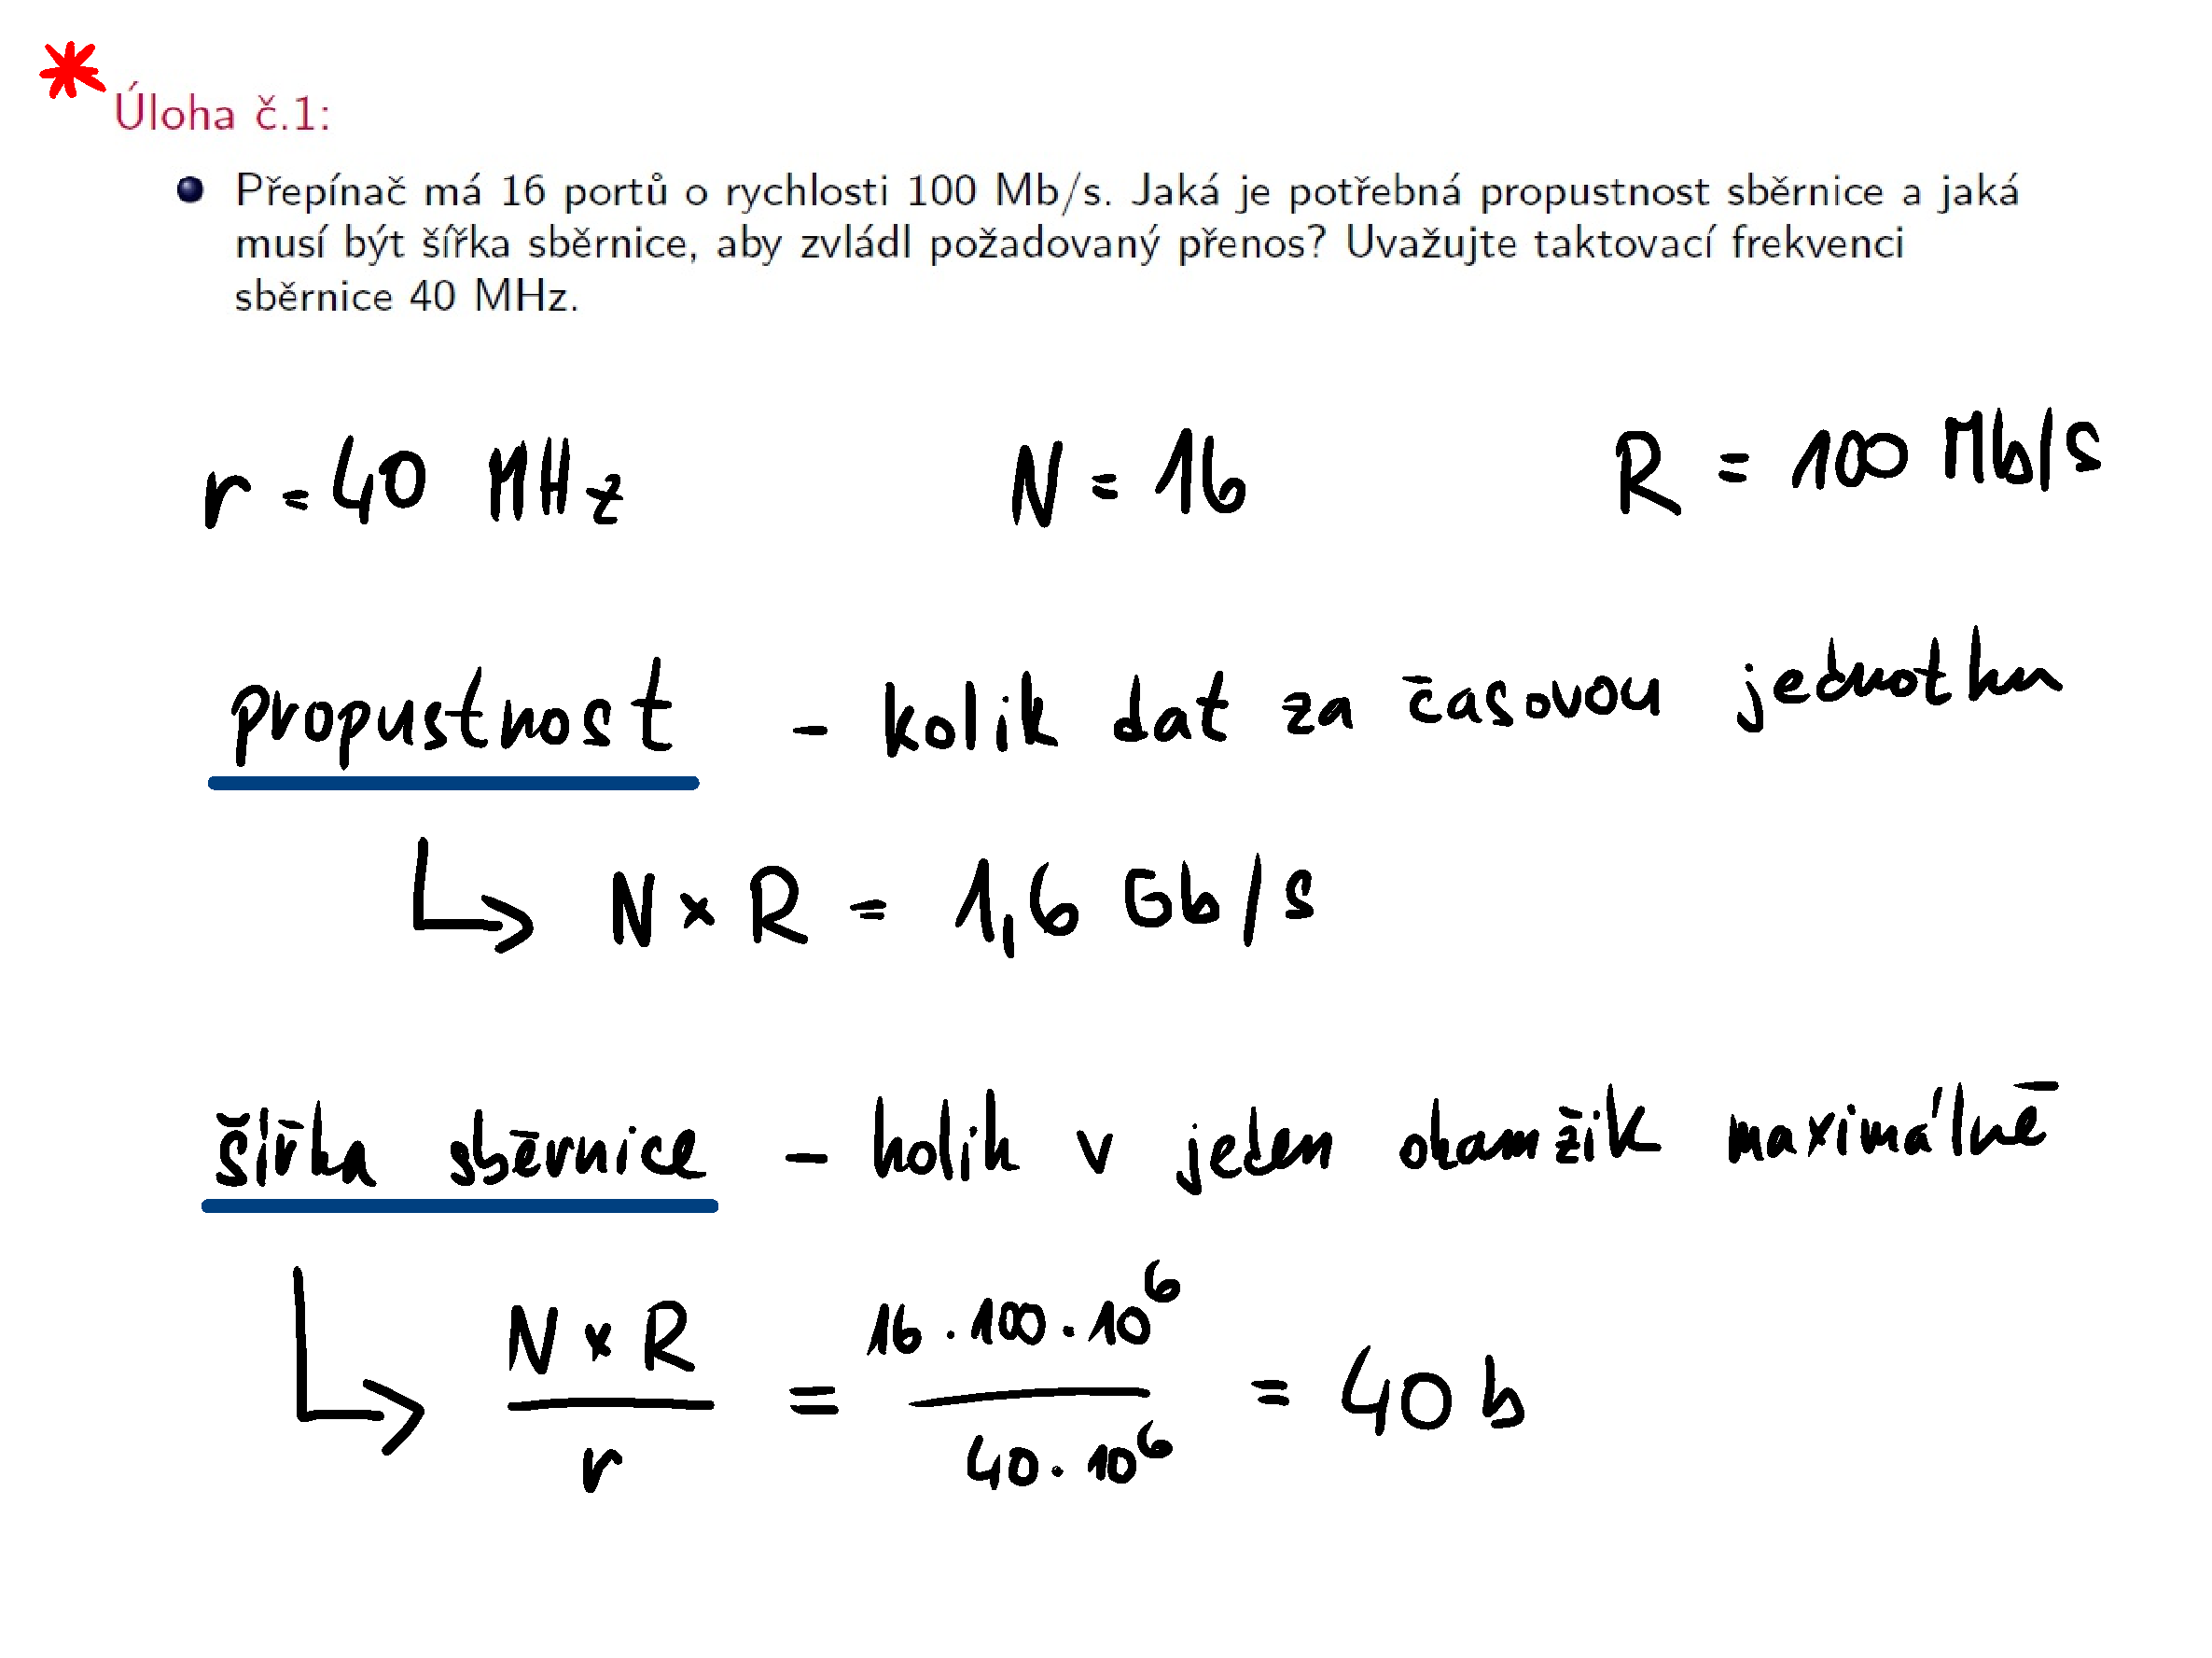
\includegraphics[width=1\linewidth]{sdilena_sbernice_priklad.pdf}
    \caption{Přepínač se sdílenou sběrnicí -- příklad.}
\end{figure}

%%%%%%%%%%%%%%%%%%%%%%%%%%%%%%%%%%%%%%%%%%%%%%%%%%%%%%%%%%%%%%%%%%%%%%%%%%%%%%%%

\section{Přepínače s přepínanou propojovací deskou (jednostupňové přepínání)}

\begin{compactitem}
    \item Umožňuje paralelní přenos rámců.
    \item Je potřeba plánovač (\textit{scheduler}), který plánuje přenos.
    \item Provedení přenosu: z bufferů vstupních karet se data přenesou do bufferů výstupních karet.
\end{compactitem}

\begin{figure}[H]
    \centering
    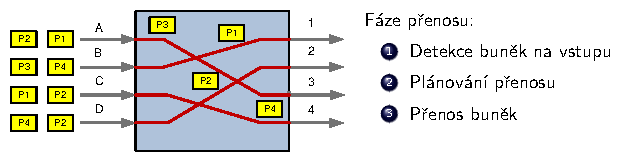
\includegraphics[width=1\linewidth]{prepinana_propojovaci_deska.pdf}
    \caption{Činnost přepínače s přepínanou propojovací deskou.}
\end{figure}

\subsection{Přepínače se sdílenou pamětí}

Sdílená paměť s fronty pro výstupní buffery

2 kroky

\todo{todo}

\subsection{Křížové přepínače}

Vnitřní blokování

\todo{todo}

\paragraph*{Algoritmus přidělování lístků} \todo{todo}

\paragraph*{Algoritmus PIM (\textit{Parallel Iterative Matching})} \todo{todo}

\paragraph*{Algoritmus iSLIP} \todo{todo}

%%%%%%%%%%%%%%%%%%%%%%%%%%%%%%%%%%%%%%%%%%%%%%%%%%%%%%%%%%%%%%%%%%%%%%%%%%%%%%%%

\section{Přepínače s přepínanou propojovací (vícestupňové přepínání)}

\todo{todo}

\subsection{Přepínací síť Clos}

\todo{todo}

\subsection{Přepínací síť Beneš}

\todo{todo}
